\section{Eigene Subscale Implementierung}
TODO MAX SCHREIB MEHR DARÜBER \\
Da der Vorgegebene Code schwer zu verstehen und lesen war, wurde versucht einen eigenen Subscale zu implementieren. Dabei wurden der Subscale in einzelne Schritte aufgesplittet, damit diese unabhängig implementiert werden können. Die einzelnen Schritte waren dabei folgende:
\begin{figure}[h]
	\centering
	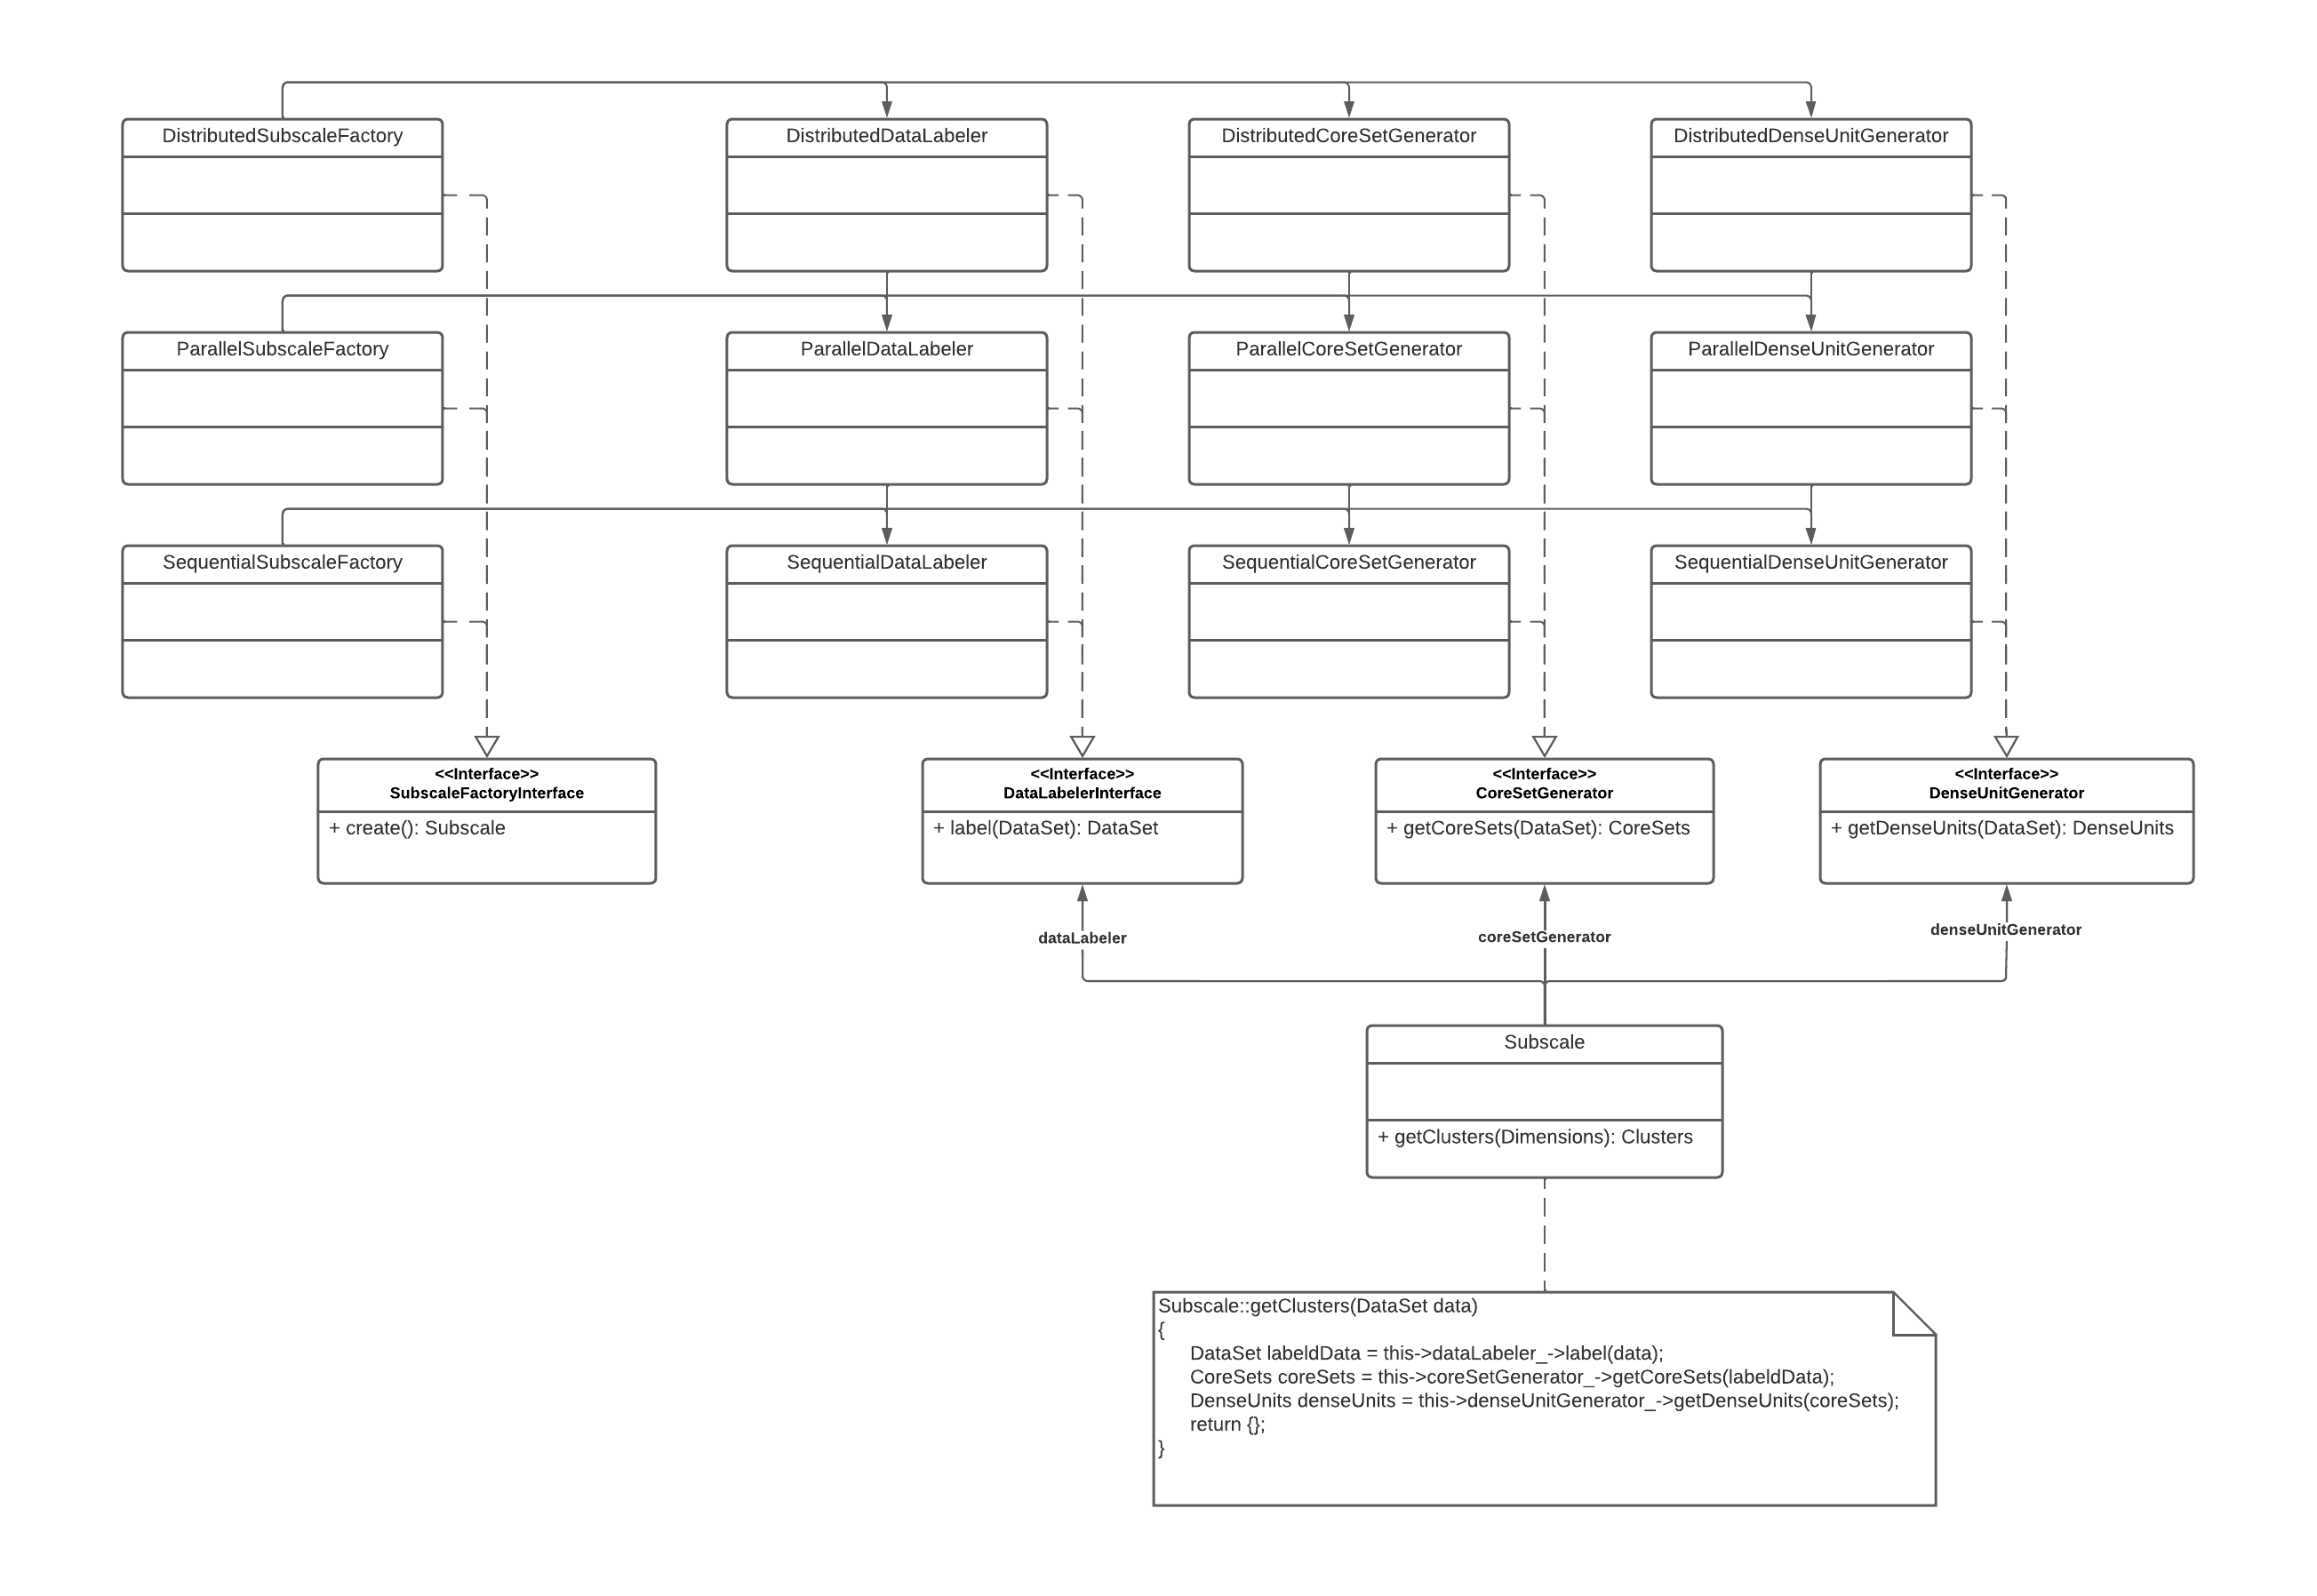
\includegraphics[width=0.7\textwidth]{./Bilder/Architektur.png}
	\caption{Architektur Subscale}
\end{figure}
\\
Während der Implementierung stellte sich raus, dass noch weitere Schritte fehlen, wie das Erkennen von Subspaces und das Kombinieren dieser Subspaces. 